\documentclass[a4paper,11pt]{report}

\usepackage[utf8]{inputenc}
\usepackage[T1]{fontenc}
\usepackage[francais]{babel}
\usepackage{amsfonts}
\usepackage{amsmath}
\usepackage{amsthm}
\usepackage{listings}
\usepackage{fullpage}
\usepackage{graphicx}

\renewcommand{\thesection}{\arabic{section}}

\newtheorem{definition}{Definition}

\title{Software Quality Assessment: Summary}
\author{Julien Delplanque}
\begin{document}
\maketitle
\newpage

\section{Assessing the quality of a software}
There are many types of quality problems that can be detected in automatically
with many tools (or plugins) and techniques. These tools can be integrated into
the IDE, integrated into the version control system, available through a
dedicated web interface or even all the preceding possibilities combined.\\

Some tools rely on \textbf{static analysis} (detecting duplicate code, detecting
dependencies, detecting structural problems) where others rely on
\textbf{dynamic analysis} (code coverage analysis, profiling).

\begin{definition}[Static analysis]
Static program analysis is the analysis of computer software that is performed
without actually executing programs.
\end{definition}

\begin{definition}[Dynamic analysis]
Dynamic program analysis is the analysis of computer software that is performed
by executing programs on a real or virtual processor.
\end{definition}

Many tools also use specific visualisation techniques.

\section{Static analysis tools}
\subsection{Detecting duplicated code}
\begin{itemize}
\item ``CBCD: Cloned Buggy Code Detector''
\item CCFinderX
\item IntelliJ IDEA 13
\item Google CodePro AnalytiX
\end{itemize}

\subsection{Code style problems and design critiques}
\begin{itemize}
\item CheckStyle
\item Google CodePro AnalytiX
\item IntelliJ IDEA 13
\item PMD
\end{itemize}

\section{Dynamic analysis tools}
\subsection{Code Coverage}
Execute the code, and check if all code (classes, methods, lines) is actually
executed. This can be used, among others to: detect obsolete or unused code,
understand which execution scenarios use which part of the code, etc\dots

\begin{itemize}
\item IntelliJ IDEA 13
\item Google CodePro AnalytiX
\end{itemize}

\subsection{Test Coverage}
Execute the tests, and check if all code (classes, methods, lines) is covered by
these tests. This can be used, among others to detect whether some parts of the
code have not been tested. Nevertheless, \textbf{test coverage is not a
sufficient criterion for test quality!}

\begin{itemize}
\item IntelliJ IDEA 13
\item Coveralls
\end{itemize}

\subsection{Code Profiling}
\begin{itemize}
\item YourKit
\end{itemize}

\section{Measuring software quality}
\subsection{Quality model}
\begin{definition}[Quality model - ISO/IEC 9126-1 standard, 2001]
Internal / External quality of a software is related to six sub-concepts:
\begin{enumerate}
\item Efficiency
\item Reliability
\item Usability
\item Portability
\item Functionality
\item Maintainability
\end{enumerate}
\end{definition}

Some of these sub-concepts have been detailed in the course:

\noindent
\textbf{Maintainability}: Analyzability, Changeability, Stability and
Testability.

\noindent
\textbf{Functionality}: Suitability, Accuracy, Interoperability and Security.

\noindent
\textbf{Usability}: Understandability, Learnability, Operability and
Attractiveness.

\noindent
\textbf{Portability}: Adaptability, Installability, Co-existence and
Replaceability.

\noindent
\textbf{Reliability}: Maturity, Fault-tolerance and Recoverability.\\

Also, the following relations are possible:

\noindent
\textbf{Maintainability} may be related to:
\begin{itemize}
\item Number of method parameters
\item Cyclomatic complexity
\item Lines of code
\item Number of error messages
\item Length of user manual
\end{itemize}

\noindent
\textbf{Reliability} may be related to:
\begin{itemize}
\item Cyclomatic complexity
\item Lines of code
\item Number of error messages
\end{itemize}

\noindent
\textbf{Portability} may be related to:
\begin{itemize}
\item Number of method parameters
\item Lines of code
\end{itemize}

\noindent
\textbf{Usability} may be related to:
\begin{itemize}
\item Number of error messages
\item Length of user manual
\end{itemize}

\clearpage
\subsection{Software metrics}
Software metrics are used to measure the internal software quality. They can be
used to identify problems with the quality of existing software systems.
There are $7$ software metrics (in the course):
\begin{enumerate}
\item size metrics,
\item coupling and cohesion metrics,
\item complexity metrics,
\item dependency metrics,
\item inheritance metrics,
\item similarity metrics ($\rightarrow$ may identify duplicated code),
\item process metrics.
\end{enumerate}

Metrics tools automate the process (separated or integrated to the IDE) and
warnings are issued when metrics values exceed a user-defined threshold.

\subsubsection{Size metric}
\begin{itemize}
\item Number Of Packages: counts the packages within the analyzed software
system.
\item Number Of Classes: counts the declared classes within the analyzed
software system.
\item Number Of Methods: counts all declared methods.
\item Lines Of Code: the number of executable source lines within the analyzed
software system.
\end{itemize}

\subsubsection{Complexity metrics}
Predictions of maintainability can be made by assessing the complexity of system
components. Studies have shown that most of the maintenance effort is spent on a
relatively small number of system components.\\

The complexity depends on: complexity of control structures, complexity of data
structures, object, method (procedure) and module size and computational
complexity (performance).

\begin{definition}[Cyclomatic complexity]
Number of independent paths in the program control flow graph. Formally, this is
the number of edges of the flow graph $-$ the number of nodes $+2$.
\end{definition}

\subsubsection{Coupling and cohesion metrics}
High cohesion between components and low coupling among components are design
principles aimed to reduce the system complexity, and as such, increase its
maintainability.\\

The principle is \textbf{``high cohesion, low coupling''}: a lower coupling
between components implies a lower impact of changes and a higher cohesion of a
component increases its understandability.

\begin{definition}[Coupling metrics]
A coupling metric measure the degree of interdependence between pairs of
components.
\end{definition}

\begin{definition}[Coupling between object classes]
Measures the number of other classes to which a given class is coupled.
``Two classes are coupled when methods declared in one class use methods or
instance variables defined by the other class.''
\end{definition}

\begin{definition}[Response for a class]
Measures the number of elements in the response set for a class = all methods
that can be invoked in response to a message to an object (instance) of the
class.
\end{definition}

\begin{definition}[FAN-OUT]
Counts the number types referenced by classes and interfaces. It only counts
those types that are not part of the same inheritance branch.
\end{definition}

There are two categories of cohesion metrics:
\begin{enumerate}
\item Cohesion metrics based on \textbf{structural} cohesion: they define and
measure structural relationships among elements belonging to the same component.
\item Cohesion metrics based on \textbf{logical} (or semantic) cohesion: do the
elements of a component logically / functionally / semantically belong together?
\end{enumerate}

\begin{definition}[Object Oriented cohesion metrics]
OO cohesion metrics measure the degree to which methods of a class belong
together. Some of these metrics are based on structural cohesion: the degree of
cohesion depends on the number of pair of methods that share or reference the
same variables and others are based on logical cohesion: requires domain
knowledge or natural language processing.
\end{definition}

\begin{definition}[Lack of cohesion in methods]
Number of methods in the class whose similarity is zero - number of methods in
the class whose similarity is non-zero.\\

Similarity between methods $m_1$ and $m_2$ is defined as the number of
instance variables used by both $m_1$ and $m_2$.
\end{definition}

\begin{definition}[FAN-OUT]
Counts the number types referenced by classes and interfaces. It only counts
those types that are not part of the same inheritance branch.
\end{definition}

\begin{definition}[Average Number of Derived Classes]
Computes the average of inherited classes. In a system of ten classes an
ANDC-value of 0.5 means, that every second class inherits from another class.
\end{definition}

\begin{definition}[Average Hierarchy Height]
Computes the average depth of the inheritance hierarchy.
\end{definition}

\noindent
\textbf{Process metrics} may be used to assess maintainability. Examples: number
of outstanding change requests, number of requests for corrective maintenance
(bug fixes), average time required for impact analysis, average time taken to
implement a change request, etc\dots An increase in any or all of these may
indicate a decreased maintainability.

\subsection{The Overview Pyramid}
The Overview Pyramid visualises software system metrics in a really compact
manner by collecting a set of metrics from the categories: inheritance, coupling
and size \& complexity, and putting them into relation.\\

\begin{figure}[h]
\center
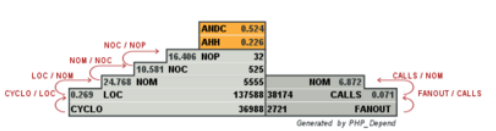
\includegraphics[width=.5\textwidth]{figures/overview_pyramid.png}
\end{figure}

Individual metrics values can be computed and related by computing average
values (e.g. LOC/NOM = average lines of code per method, NOC/NOP = average
number of classes per package, etc\dots). Then, these metrics values can be
compared against reference values to determine the quality of a particular
software.

\subsection{More tool support}
\subsubsection{Counting - CLOC}
Counts blank lines, comment lines, and physical lines of source code in many
programming language. Given two code versions, computes differences in blank,
comment, and source lines.

\subsubsection{CodePro AnalytiX}
Has a support for metrics.

\subsubsection{SDMetrics}
Computes metrics for UML models.

\end{document}
